%%%%%%%%%%%%%%%%%%%%%%%%%%%%%%%%%%%%%%%%%%%%%%%%%%%%%%%%%%%%%%%%%%%
%%% Documento LaTeX 																						%%%
%%%%%%%%%%%%%%%%%%%%%%%%%%%%%%%%%%%%%%%%%%%%%%%%%%%%%%%%%%%%%%%%%%%
% Título:		Capítulo 3
% Autor:  	Ignacio Moreno Doblas
% Fecha:  	2014-02-01, actualizado 2019-11-11
% Versión:	0.5.0
%%%%%%%%%%%%%%%%%%%%%%%%%%%%%%%%%%%%%%%%%%%%%%%%%%%%%%%%%%%%%%%%%%%
% !TEX root = A0.MiTFG.tex

\section{Quinta iteración: Consideraciones de diseño}
    \subsection{Resumen}
    
        Una vez teniendo el proyecto funcionando con todas las funciones básicas implementadas ha llegado el momento de frenar el desarrollo de nuevas funcionalidades y echar la vista atrás con el fin de mejorar el acabado general del proyecto.
        
        En esta iteración se llevarán a cabo tareas relacionadas con facilitar la lectura del código y mejorar el aspecto visual y usabilidad de la aplicación de usuario.
    
    \subsection{Requisitos}
    
        A diferencia de las anteriores, en esta iteración no se satisface ningún requisito en particular, pero igualmente se puede dividir el trabajo en las siguientes tareas.
        
        \begin{enumerate}
            \item Limpieza de código y asegurar coherencia en la nomenclatura.
            \item Añadir comentarios necesarios para facilitar la lectura del código y su mantenimiento.
            \item Mejorar la apariencia visual del panel y mejorar su usabilidad en la medida de lo posible.
        \end{enumerate}
    \subsection{Desarrollo}
    
        Para la primera tarea, \textit{revisar la limpieza del código y su coherencia}, se recorren los diferentes ficheros del código examinando con detalle el estilo de escritura utilizado, garantizando un código estandarizado y que satisfaga las consideraciones de diseño establecidas al comienzo del desarrollo.
        
       \textit{Comentarios explicativos} se han añadido a las declaraciones y demás elementos del código con el objetivo de facilitar la comprensión del mismo, especialmente en las zonas destinadas a ser modificadas por el usuario final. Además se han añadido comentarios referidos a posibles mejoras y correcciones que se podrían implementar en un futuro, por si el sistema sigue desarrollándose una vez concluido este proyecto. Minimizando así el tiempo de estudio previo a comenzar a realizar modificaciones.
       
       Para \textit{mejorar el apartado visual del panel} se han redistribuido los elementos ya expuestos en este proyecto, agrupándolos por secciones. Para \textit{mejorar la usabilidad} se han incluido textos descriptivos detallando a que corresponde cada elemento del panel y una nueva funcionalidad que permite detener el envío de una señal para realizar el análisis de otra sin la necesidad de reiniciar el panel. La nueva disposición de los elementos puede observarse en las imágenes \ref{fig:EndConfig} y \ref{fig:EndResults}.
       
       \begin{figure}[H]
            \centering
                    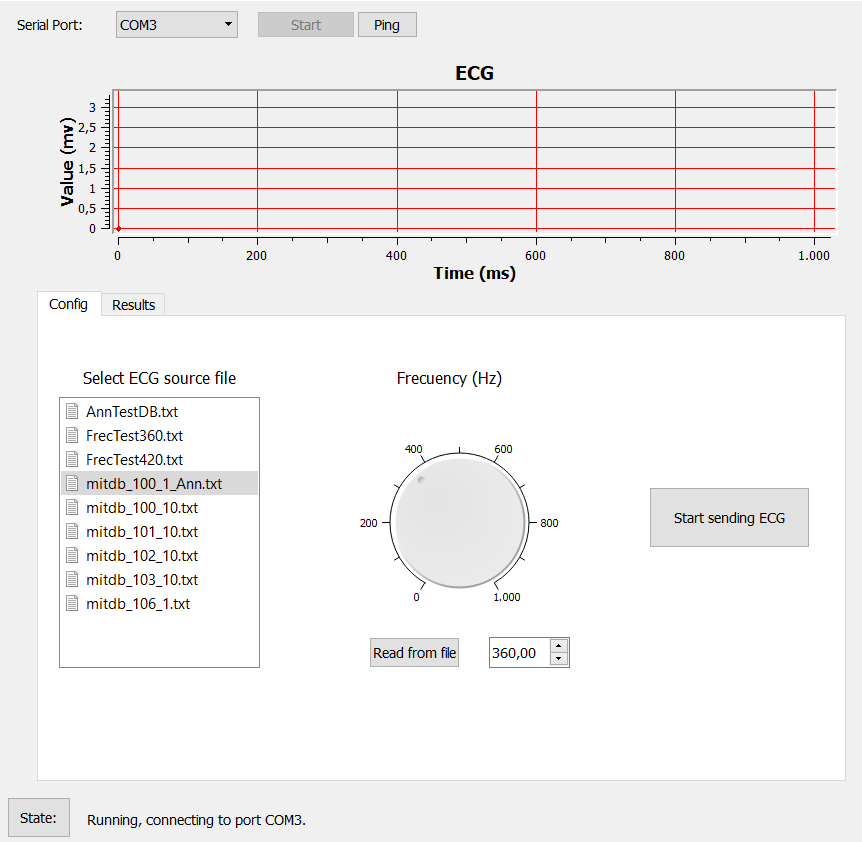
\includegraphics[width = \linewidth]{figuras/Config.PNG}
            \caption{Panel de usuario, configuración de la prueba.}
            \label{fig:EndConfig}
        \end{figure}
        
        \begin{figure}[H]
            \centering
                    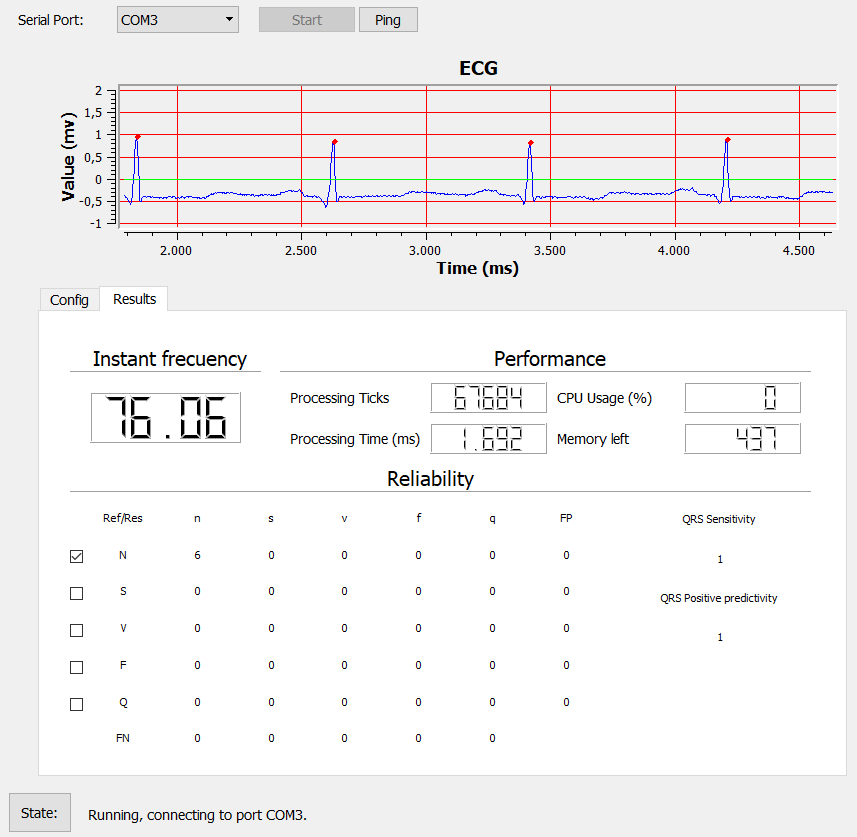
\includegraphics[width = \linewidth]{figuras/Results.PNG}
            \caption{Panel de usuario, resultados de la prueba.}
            \label{fig:EndResults}
        \end{figure}
       
    \subsection{Pruebas}
    
    En esta iteración la única funcionalidad implementada susceptible de contener errores es la gestión del estado, necesaria para permitir al usuario detener y comenzar pruebas con diferentes muestras sin la necesidad de cerrar la sesión. Dado el carácter integral de esta funcionalidad resulta muy complicado realizar test unitarios, por lo que el método de prueba empleado ha sido simplemente un debug intensivo probando exhaustivamente los casos posibles.
    
    \subsection{Conclusiones}
    
    Con esta iteración queda finalizado el desarrollo de este proyecto. El estado actual del sistema es estable, funcional y medianamente usable por lo que se pueden dar por finalizados todos los requisitos de alta prioridad establecidos al inicio del proyecto. Si bien hay aspectos del sistema que pueden ser mejorados y elementos que pueden añadirse, están fuera del alcance de este proyecto, aunque se hablará sobre ellos en las conclusiones generales del proyecto en un apartado posterior.